\documentclass[../tesis_main.text]{subfiles}

\chapter{Manipulador}
	En esta sección se hablará de las caracteriscias mecánicas del brazo robótico ensamblado en el robot de servicio Justina. Se describirán los elementos que componen el brazo robótico haciendo enfasís en la ubicación de los actuadores y como influye esto en el modelo matematico del mismo.


%%%%%%%%%%%%%%%%%%%%%%%%%%%%%%%%%%%%%%%%%%%%%%%%%%%%%%%%%%%%%%%%
           %%%%%%  DESCRPCIÓN SERVOMOTORES   %%%%%%%%
%%%%%%%%%%%%%%%%%%%%%%%%%%%%%%%%%%%%%%%%%%%%%%%%%%%%%%%%%%%%%%%%
	\section{Documentación servos dynamixel}
		Los servomotores Dynamixel son un sistema de actuador inteligente desarrollados con el propósito de funcionar como uniones de conexión en un robot o estructura mecánica. Los servomotores Dynamixel están diseñados para ser modulares y soportar la conexión en cadena en cualquier robot o diseño mecánico. Este tipo de servomotores es popular por los beneficios que ofrece: movimientos robóticos potentes y flexibles.\\

		El conjunto de servomotores Dynamixel son un grupo de actuadores de alto rendimiento con reductor, controlador y un protocolo de red completamente integrados en un módulo de servomotor programable y en red. El estado del actuador se puede leer y monitorear a través de un flujo de paquetes de datos. \cite{dynamixelEpage}\\

		Los servomotores de la marca Dynamixel, cuentan con diferentes gamas de productos de acuerdo a las necesidades de cada proyecto. El brazo robótico referente a este documento está constituido unicamente por motores de la gama MX, de la cual se describen las caracteristicas más sobresalientes a continuación.\\  

			\subsection{Motores dynamixel Serie MX}
		Los actuadores dynamixel de la serie MX pertencen a la última generación de actuadores de la companñia Robotis Dynamixel. Están equipados con un procesador Cortex M3 de 32 bits a 72 mhz, un encoder magnético sin contacto con una resolución 4 veces mayor que la serie AX / RX, además ofrecen una velocidad de comunicación de hasta 3 mbps con el nuevo bus TTL 2.0. Cada servomotor cuenta con la capacidad  de monitorear su velocidad, temperatura, posición del eje, voltaje y carga.\\

		Por otro lado los motores Dynamixel de la seire MX cuentan con la implemntación de un algoritmo de control PID para mantener la posición del eje. Las ganancias del algoritmo de control PID se pueden ajustar individualmente para cada servo, lo que le permite controlar la velocidad y la fuerza de la respuesta del motor. Todos los servos de la serie MX usan un voltaje nominal de 12v. La característica más importante de esta seie de servomotores es que la gestión de la información proveniente del sensor y la ejecución del algoritmo de control de posición son manejados por el microcontrolador integrado del servo. Este enfoque distribuido deja a su controlador principal libre para realizar otras funciones.\\


		En lo que respecta a la parte mecánica, todos los servos DYNAMIXEL son compatibles con una amplia variedad de bridas, acoplamientos y sujetadores lo cual facilita la construcción de cualquier configuración deseada. Este conjunto de elementos mecánicos permite una conección directa cualquier modelo de servomotores DYNAMIXEL, lo que le permite una gran variedad de configuraciones para cualquier necesidad. Dada la gran variedad de configuraciones, este tipo de elementos de unión y fijación resultó de gran ayuda mecánica al momento de contruir el brazo robótico donde se implentaron los algoritmos descritos en el presente trabajo.\\

		\begin{figure}[h!]
			\begin{center}
			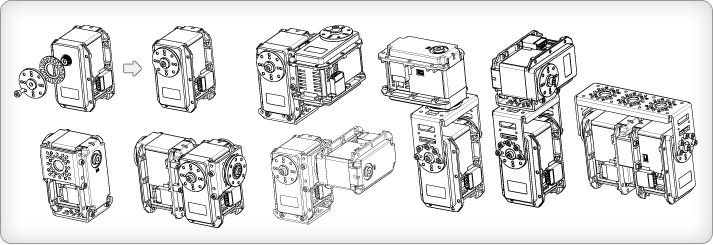
\includegraphics[width=14.5cm, height=6.5cm]{/dynamixel_conexions.jpg}	
			\caption{Variedad de ensambles para servomotores.}
			\end{center}
		\end{figure}

		Resuminedo las características de los sermovomotores de la serie MX, podemos enlistar las siguientes:\\ 

		\begin{itemize}
			\item{Movimiento sin contacto y detección de posición.}
			\item{Interfaz de comunicación TTL estándar.}
			\item{Comunicación de alta velocidad de hasta 4.5 Mbps.}
			\item{Control PID para autocorrección en posicionamiento.}
			\item{Control de par basado en corriente (4096 steps, 2.69mA/step)}
			\item{Ahorro de energía (corriente reducida de 100 mA a 40 mA)}
		\end{itemize}

		Si desea controlar este servo DYNAMIXEL desde un equipo de computo es necesario contar con un dispositivo que facilite la comunicación entre este y el microprocesador de cada uno de los servomotores, el dispositivo que cumple con esta funcionalidad es el USB2Dynamixel.\\

		El controlador USB2Dynamixel se conecta al puerto USB en una computadora y tiene un puerto de 3 y 4 pines para conectar Dynamixels. El USB2Dynamixel se puede usar con controladores como CM-5 y CM-2 que usan comunicación en serie, además soporta la comunicación en cadena propia de los servomotores Dynamixel. Es impornate mencionar que este dispositivo posee un interruptor para seleccionar entre diferentes protocolos de comunicación: RS-232, RS-485, TTL. Por tanto consta de:\\

		\begin{itemize}
			\item{Conector 3P: puerto de comunicación para nivel TTL (para control de serie AX y MX)}
			\item{Conector 4P: puerto de comunicación RS-485 (para control de serie DX, RX, EX y MX)}
		\end{itemize}


		\begin{figure}[h!]
			\begin{center}
			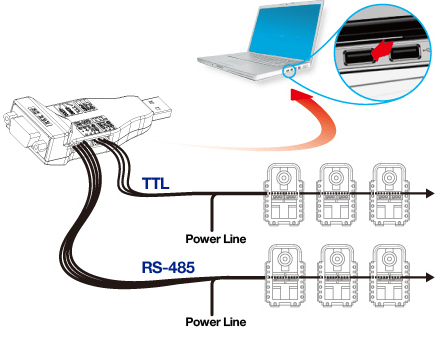
\includegraphics[width=10.5cm, height=8.5cm]{/usb2dynamixel.jpg}	
			\caption{Dispositivo de comunicación USB a protocolo serial.}
			\end{center}
		\end{figure}

		Los motores que componen esta gama comparten caracteristicas, las cuales se menacionan a continuación:\\

\begin{tabular}{ |p{6.5cm}||p{2.1cm}|p{2.1cm}|p{2.1cm}|  }
 \hline
 \multicolumn{4}{|c|}{\textbf{MOTORES GAMA MX} } \\
 \hline
 Voltaje de operación  &  14.8v   &	   12v   &   11.1v\\
 \hline
 Protocolo             &  \multicolumn{3}{|c|}{TTL Serial Asincrono} \\
 \hline
 Velocidad del puerto  &  \multicolumn{3}{|c|}{8000bps - 3Mbps} \\
 \hline
 Retroalimentación de posición & \multicolumn{3}{|c|}{ SI} \\
 \hline
 Retroalimentación de temperatura & \multicolumn{3}{|c|}{ SI}\\
 \hline
 Control PID           & \multicolumn{3}{|c|}{ SI } \\
 \hline
 Material              & \multicolumn{3}{|c|}{ Carcasa platica y reducción metálica} \\
 \hline
 Motor                 & \multicolumn{3}{|c|}{ Maxon RE-MAX} \\
 \hline
\end{tabular}\\

		Los modelos de motores que componen esta gama difieren en caracteríticas tales como las dimensiones, el par máximno a rotor bloqueado, la corriente máxima, o la velocidad máxima. A continuación se en listan las características más sobresalientes para cada modelo de motor.\\ 


		\subsection{Características MX-106}

\begin{tabular}{ |p{6.5cm}||p{2.1cm}|p{2.1cm}|p{2.1cm}|  }
 \hline
 \multicolumn{4}{|c|}{\textbf{MX-106} } \\
 \hline
 Voltaje de operación  &  14.8v   &	   12v   &   11.1v\\
 \hline
 Par de bloqueo        &  102kg.cm  &  85.6kg.cm  &  81.5kg.cm\\
 Velocidad sin carga   &  55rpm     &  45rpm      &  41rpm\\
 \hline
 Peso                  &  \multicolumn{3}{|c|}{153g} \\
 \hline
 Tamaño                &  \multicolumn{3}{|c|}{40.2 x 65.1 x 46 mm} \\
 \hline
 Resolución            &  \multicolumn{3}{|c|}{ 0.088 grado/valor de registro} \\
 \hline
 Relación de reducción &  \multicolumn{3}{|c|}{1/200} \\
 \hline
 Corriente máxima      &  \multicolumn{3}{|c|}{5.2A @ 12V} \\
 \hline
\end{tabular}

\begin{figure}[h!]
	\begin{center}
	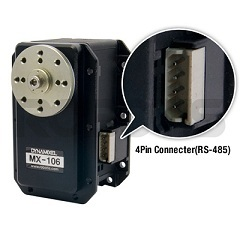
\includegraphics[width=8.5cm, height=8.5cm]{/MX_106R_2.jpg}	
	\caption{Servomotor dynamixel modelo MX-106.}
	\end{center}
\end{figure}


		\subsection{Características MX-64}

\begin{tabular}{ |p{6.5cm}||p{2.1cm}|p{2.1cm}|p{2.1cm}|  }
 \hline
 \multicolumn{4}{|c|}{\textbf{MX-64} } \\
 \hline
 Voltaje de operación  &  14.8v   &	   12v   &   11.1v\\
 \hline
 Par de bloqueo        &  74kg.cm   &  61kg.cm   &  56kg.cm\\
 Velocidad sin carga   &  78rpm     &  63rpm     &  58rpm\\
 \hline
 Peso                  &  \multicolumn{3}{|c|}{126g} \\
 \hline
 Tamaño                &  \multicolumn{3}{|c|}{40.2 x 61.1 x 41 mm} \\
 \hline
 Resolución            &  \multicolumn{3}{|c|}{ 0.088 grado/valor de registro} \\
 \hline
 Relación de reducción &  \multicolumn{3}{|c|}{1/200} \\
 \hline
 Corriente máxima      &  \multicolumn{3}{|c|}{4.1A @ 12V} \\
 \hline
\end{tabular}

\begin{figure}[h!]
	\begin{center}
	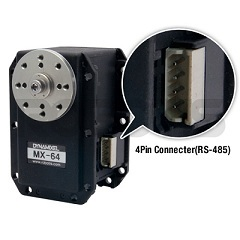
\includegraphics[width=8.5cm, height=8.5cm]{/MX_64R_2.jpg}	
	\caption{Servomotor dynamixel modelo MX-64.}
	\end{center}
\end{figure}

		\subsection{Características MX-28}

\begin{tabular}{ |p{6.5cm}||p{2.1cm}|p{2.1cm}|p{2.1cm}|  }
 \hline
 \multicolumn{4}{|c|}{\textbf{MX-28} } \\
 \hline
 Voltaje de operación  &  14.8v   &	   12v   &   11.1v\\
 \hline
 Par de bloqueo        &  31.6kg.cm  &  25.5kg.cm   &  23.4kg.cm\\
 Velocidad sin carga   &  67rpm      &  55rpm       &  50rpm\\
 \hline
 Peso                  &  \multicolumn{3}{|c|}{72g} \\
 \hline
 Tamaño                &  \multicolumn{3}{|c|}{35.6 x 50.6 x 35.5 mm} \\
 \hline
 Resolución            &  \multicolumn{3}{|c|}{ 0.088 grado/valor de registro} \\
 \hline
 Relación de reducción &  \multicolumn{3}{|c|}{1/193} \\
 \hline
 Corriente máxima      &  \multicolumn{3}{|c|}{1.4A @ 12V} \\
 \hline
\end{tabular}

\begin{figure}[h!]
	\begin{center}
	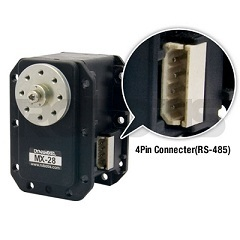
\includegraphics[width=8.5cm, height=8.5cm]{/MX_28R_2.jpg}	
	\caption{Servomotor dynamixel modelo MX-64.}
	\end{center}
\end{figure}


		\subsection{Caracteristicas de conexión}







%%%%%%%%%%%%%%%%%%%%%%%%%%%%%%%%%%%%%%%%%%%%%%%%%%%%%%%%%%
%%%%%%%%%%%%%%% DESCRIPCION DEL HARDWARE %%%%%%%%%%%%%%%%%
%%%%%%%%%%%%%%%%%%%%%%%%%%%%%%%%%%%%%%%%%%%%%%%%%%%%%%%%%%

	\section{Descripción de los elementos del sistema de manipulación}
		El sistema de Hardware del brazo robótico está compuesto por servomotores Dynamixel fabricados por la compañía Robotis (***cite Robotis Official page). Eta compañia cuenta con diversas gamas de modelos de servomotores según las necesidades de la apliación. A continuación se describirá el sistema en orden descendente.\\

		**Imagen del brazo resaltando servomotores...\\


		En la parte superior del brazo robótico se encuentran dos servomotores Dynamixel MX-106 conectados como maestro-esclavo, configurados en este modo trabajan de manera conjunta aumentando el par unitario de cada uno de los servos. Dadas las caracteristicas antes descritas en la tabla [] podemos observar que la configuración de servomotores entrega un par de torsión máximo de *****... El sentido de giro positivo del arreglo de servomotores es el mostrado en la figura []. \\

		Posteriormente se encuentra un servomotor modelo MX-106 


		**** Cadena completa y muestra de las conexiones electricas (comparación antes y despues.) 





	

%%%%%%%%%%%%%%%%%%%%%%%%%%%%%%%%%%%%%%%%%%%%%%%%%%%%%%%%%%%%%%%%
              %%%%%%  CINEMATICA DIRECTA   %%%%%%%%
%%%%%%%%%%%%%%%%%%%%%%%%%%%%%%%%%%%%%%%%%%%%%%%%%%%%%%%%%%%%%%%%

	\section{Cinemática directa}
		**** Teoría trasformaciones y medidas del brazo robotico
		**** Implementación (Descrpción con ROS)







%%%%%%%%%%%%%%%%%%%%%%%%%%%%%%%%%%%%%%%%%%%%%%%%%%%%%%%%%%%%%%%%
              %%%%%%  CINEMATICA INVERSA   %%%%%%%%
%%%%%%%%%%%%%%%%%%%%%%%%%%%%%%%%%%%%%%%%%%%%%%%%%%%%%%%%%%%%%%%%
	\section{Cinemática inversa}
